
\documentclass{article}

\usepackage{listings}
\usepackage{graphicx}
\usepackage{hyperref}

\hypersetup{colorlinks,linkcolor=,urlcolor=blue}

\begin{document}

\begin{verbatim}
Company was chosen, ex. IBM.
Script was written to extract relations from finance.google.com.
Script is intended to run many times, so it caches request results in files.
Traverse depth and relation count per company can be tuned.
With 3 relations network stops expanding at depth 16 giving 73 nodes.

Graph was visualized in Gephi.
Layout "Force Atlas" was applied.
Graph was partitioned by color (statistics: modularity: resolution 5).
It looks like companies form groups by industry:
    computers, software, telecom, chip.
Size of nodes was set (ranking) according to their degree.
This looks like showing main companies inside groups:
    TI and Intel, HP, MS and Oracle.
However on setting size by betweeness centrality (statistics: avg. path length)
    Apple inc. become the largest integrator.

No sensible way to handle this network data in PAST was found.

\end{verbatim}

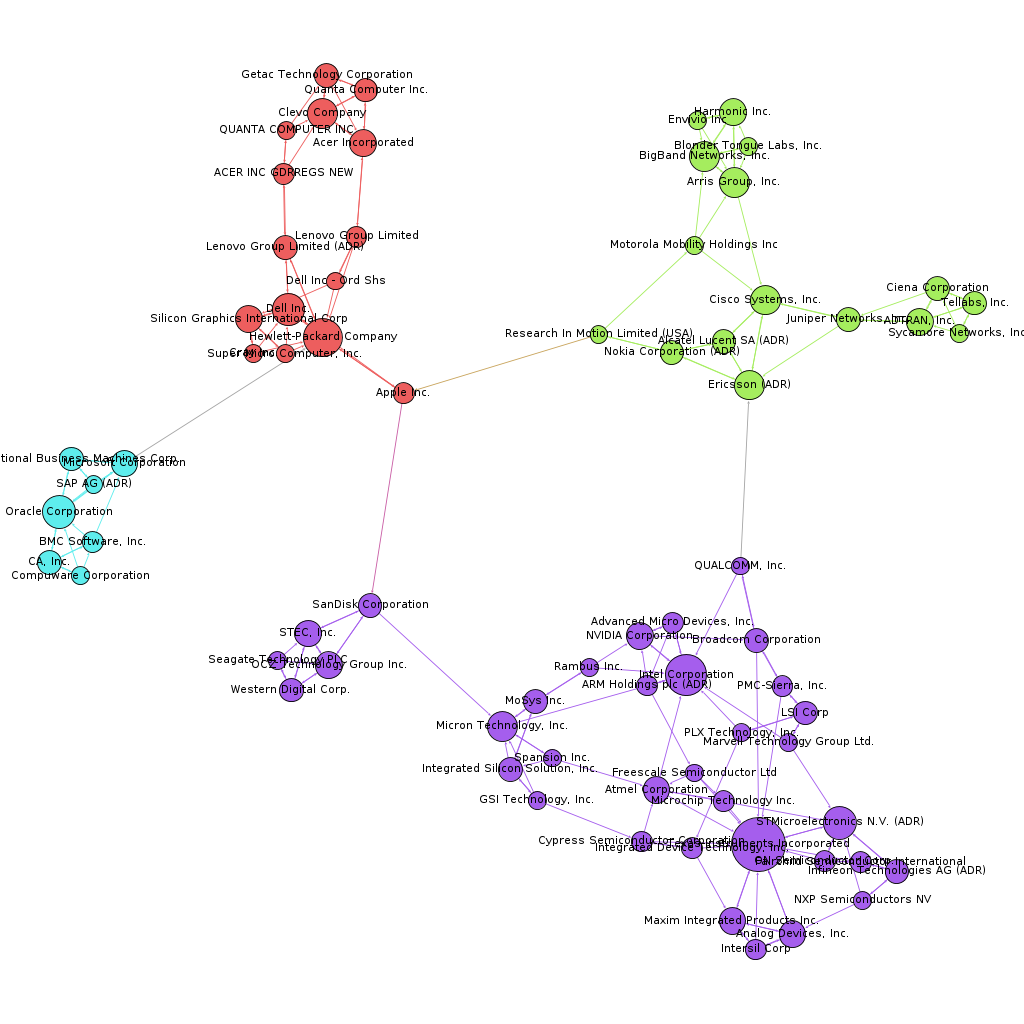
\includegraphics[width=100mm]{itcomp.png}

\clearpage

See perl sources at \url{https://github.com/rewlad/ttu_andm}

\lstinputlisting[language=Perl,numbers=left,basicstyle=\footnotesize\ttfamily,breaklines=true]{geta.pl}

\end{document}